\chapter{Descripción de la Solución}

% Involucra todos o algunos de los siguientes:
% - Arquitectura del software
% - Arquitectura del hardware
% - Diseño de la base de datos
% - Diseño de clases
% - Diseño de estructuras de datos
% - Diseño de algoritmos
% - Diseño de la interfaz de usuario
% Justificación y descripción de cómo la solución resuelve el problema planteado

A continuación se describe la solución implementada para el presente proyecto. Se detalla aquí la estructura, diseño y funcionamiento del sistema y la aplicación realizados con el fin de cumplir con los requerimientos descritos anteriormente.

\section{Arquitectura de software}

Dado que, para fines del proyecto, se requería de una herramienta con la cual se puediese llevar a cabo una serie de pruebas en distintos contextos, se optó por dividir el sistema en dos paquetes distintos; cada uno con una función específica, e interfaces bien definidas, con el fin de facilitar su posterior extensión y reutilización. En la Figura \ref{fig:arq_sistema} se muestra un diagrama con la arquitectura general del sistema.

\begin{figure}[h!]
\begin{center}
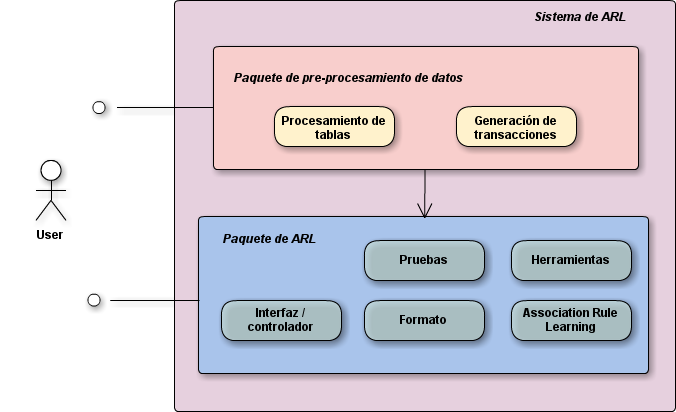
\includegraphics[width=0.9\textwidth]{imagenes/arq_sistema.png}
\end{center}
\vspace*{-5mm}
\caption{Diagrama de la arquitectura del sistema, con sus paquetes y módulos principales.}
\label{fig:arq_sistema}
\end{figure}

A continuación se detallan sus paquetes, módulos, e interfaces y explica sus funciones.

\subsection{Paquete de Association Rule Learning (ARL)}

El paquete de \textit{Association Rule Learning (ARL)} es el encargado de realizar el aprendizaje mediante reglas de asociación en sí; vale decir, de recibir un conjunto de datos con transacciones y de retornar reglas de asociación generadas a partir de aquel conjunto.

En las siguientes secciones se espacifican los formatos de entrada y salida de este paquete junto con una descripción de los módulos que lo componen.

\subsubsection{Módulo de interfaz de usuario/controlador}

El módulo de interfaz de usuario y controlador es el encargado de recibir directamente del usuario los parámetros de entrada correspondientes. Este módulo contiene métodos, clases y funciones que reciben los parámetros del usuario, abren y leen los archivos de entrada adecuados, los procesan de acuerdo al formato especificado, y hacen entrega de los datos al módulo principal de ARL.

Este módulo, es el encargado, además de recibir las reglas de asociación, entregarlas al módulo de formato para luego retornarlas al usuario en un archivo correspondiente.

\subsubsection{Módulo de formato}

Es el módulo encargado de analizar los archivos de entrada leídos por el módulo de interfaz de usuario, extraer la información pertinente de ellos según el formato especificado, y retornar los datos en una estructura adecuada para luego ser procesados por el módulo principal de ARL. A su vez, este módulo realiza, además la labor inversa; vale decir, recibe las reglas de asociación en una estructura de datos estándar para luego entregarlas al módulo de interfaz en el formato requerido por el usuario.

Hasta el momento los formatos soportados son valores separados por coma, o \textit{comma separated values (CSV)} para archivos de entrada, y CSV o tabla en formato \LaTeX\ para archivos de salida.

\subsubsection{Módulo principal de ARL}

El módulo principal de ARL es el encargado de llevar a cabo el algoritmo de aprendizaje mediante reglas de asociación en sí. En su parte lógica, consta de dos sub-módulos principales. El primero es es sub-módulo encargado de extraer los conjuntos de ítemes frecuentes; vale decir, aquellos que cumplen con el requerimiento de soporte mínimo. Y el segundo es el sub-módulo de generación de reglas, que es el encargado de recibir los conjuntos de ítemes frecuentes y generar, a partir de ellos, las reglas de asociación que cumplen con el requerimiento de confianza mínima indicado.

\subsubsection{Módulo de testeo de ARL}

Se encuentra dentro de este paquete, además, un módulo de testeo de los algoritmos de ARL sobre datos de prueba de pequeña envergadura; con el fin de realizar chequeos periódicos del funcionamiento correcto de estos algoritmos en la medida que se realizan cambios, mejoras o refactorizaciones sobre su código fuente.

\subsubsection{Módulo de herramientas}

Finalmente, se encuentra el módulo de herramientas generales, que consta de una serie de funciones de uso frecuente por parte de otros módulos del paquete; tales como operaciones sobre listas anidadas, búsqueda de llaves sobre diccionarios específicos, entre otros.

\subsection{Paquete de procesamiento de datos}

Debido a que, en la mayoría de las ocasiones los datos sobre los cuales se desea aplicar los algoritmos de reglas de asociación no se encuentran desde un comienzo en los formatos o estructuras necesarias, se procedió a implementar un paquete de pre-procesamiento. Este contiene una serie de scripts y métodos cuya función principal es extraer los datos desde sus fuentes originales, opcionalmente inferir aquella información que sea relevante, y guardarla en archivos cuyo formato sea comprensible para el paquete de aprendizaje de reglas de asociación.

En su implementación actual, este paquete se encuentra enfocado, en su mayor parte, para trabajar sobre datos extraídos a partir del Sloan Digital Sky Survey (SDSS).

A continuación se enumeran algunos de sus componentes más importantes.

\subsubsection{Queries SQL}

Una colección de queries relevantes para ejecutar en las bases de datos de SDSS y extraer los datos sobre los cuales obtener las reglas de asociación.

\subsubsection{Módulo de procesamiento de tablas}

Contiene una serie de scripts cuyo fin es recibir un archivo de tabla de base de datos en formato CSV y procesar los datos que contiene; por ejemplo, eliminando ciertas filas, añadiendo columnas calculadas a partir de las ya existentes, entre otros. Los resultados son guardados en un nuevo archivo de tabla en formato CSV.

\subsubsection{Módulo de generación de transacciones}

Este módulo contiene scripts cuya función es recibir un archivo de tabla de base de datos en formato CSV, y a partir de él generar un archivo CSV que contenga una transacción por cada fila; cada una de estas con una lista de ítemes en formato adecuado para ser recibido por el paquete de ARL.

\section{Diseño de clases}

En la Figura \ref{fig:arl_diag_clases} se observa un diagrama con las clases más importantes dentro del paquete de Association Rule Learning y sus relaciones.

\begin{figure}[h!]
\begin{center}
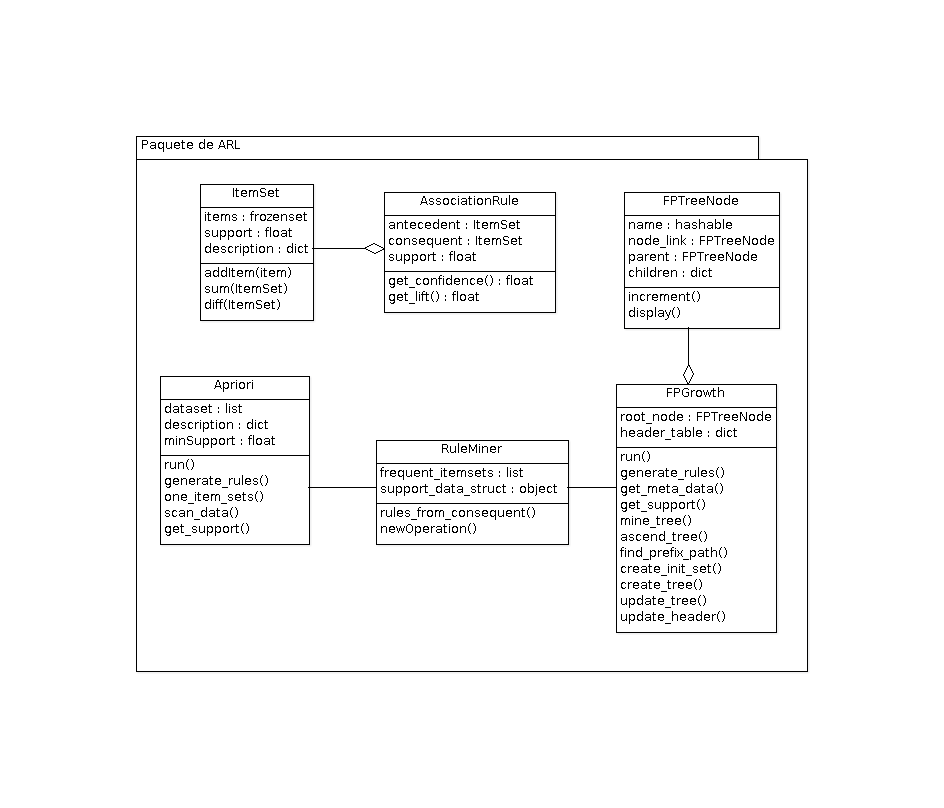
\includegraphics[width=0.9\textwidth]{imagenes/arl_diag_clases.png}
\end{center}
\vspace*{-5mm}
\caption{Diagrama de clases más importantes del paquete de ARL.}
\label{fig:arl_diag_clases}
\end{figure}

A continuación se detallan las clases de objetos más importantes del sistema.

\subsection{Clase \textit{ItemSet}}

La clase \textit{ItemSet} es la encargada de mantener información sobre un conjunto de ítemes y abstraer su estructura de datos subyacente. Cada instancia de esta clase corresponde a un conjunto de ítemes distinto, y contiene campos que guardan la información más reciente sobre su soporte (calculado sobre un cierto conjunto de transacciones) y punteros a meta-datos con información adicional sobre los ítemes en sí. Su interfaz asegura que se pueda realizar de forma adecuada, visto desde un punto de vista matemáticamente abstracto, las operaciones más comúnes de conjuntos de elementos; como comprobar pertenencia, sumar de conjuntos, diferencia entre conjuntos, entre otros.

\subsection{Clase \textit{AssociationRule}}

La clase \textit{AssociationRule} es la que define la estructura y comportamiento de las reglas de asociación. Cada instancia de esta clase corresponde a una regla de asociación en particular, extraída a partir de un cierto conjunto de datos. Cada regla de asociación consta de dos objetos de la clase \textit{ItemSet}; uno para el antecedente y otro para el consecuente de la regla. Además contiene un campo que codifica su soporte, junto con métodos para calcular sus medidas de relevancia, tales como su confianza y lift.

\subsection{Clase \textit{FrequentItemSetMiner}}

La clase \textit{FrequentItemSetMiner} es la encargada de abstraer y guardar información sobre el proceso de extraer a partir de las transacciones aquellos conjuntos de ítemes que cumplan con un requisito de soporte mínimo dado. Cada instancia de esta clase corresponde a un proceso de estracción distinto, conteniendo campos y estructuras de datos para los algoritmos involucrados, su estado actual y su resultado.

En su implementación actual, esta clase es heredada por dos sub-clases. Una correspondiente al algoritmo \textit{Apriori}, y otra al algoritmo \textit{FP-Growth}. Cada una contiene su propia implementación de los métodos principales, definidos en su clase padre, junto con sus propias funciones auxiliares y estructuras de datos correspondientes.

\subsection{Clase \textit{RuleMiner}}

La clase \textit{RuleMiner} es la que abstrae el proceso de extraer reglas de asociación a partir de conjuntos frecuentes de ítemes. Cada instancia de esta clase corresponde a un proceso de extracción distinto; básicamente el mismo en todo los casos salvo en ciertos detalles, como algunas funciones auxiliares y referencias a estructuras de datos, dependiendo de si los conjuntos fueron extraídos mediante \textit{Apriori} o \textit{FP-Growth}.

\section{Detalles de implementación}

La implementación del sistema se llevó a cabo en el lenguaje de programación Python\cite{python.org}. Se realizó una implementación propia de los algoritmos antes descritos, con algunas adaptaciones para su funcionamiento correcto en el contexto de este proyecto; y se hizo uso de paquetes externos con el fin de hacer más simple el manejo de archivos CSV y la implementación de la interfaz por línea de comando.

\subsection{Extracción de conjuntos de ítemes frecuentes}

Para la extracción de conjuntos de ítemes frecuentes se procedió a realizar la implementación de los algoritmos \textit{Apriori} y \textit{FP-Growth}. Ambos algoritmos reciben las transacciones en una misma estructura de datos y retornan los conjuntos frecuentes también en una misma estructura en ambos casos. Pero cada una de estas clases posee sus propios métodos, definidos por los algoritmos en general.

En general, para ambos algoritmos la estructura de datos más utilizada para la implementación subyacente en los objetos correspondientes a conjuntos frecuentes, candidatos, antecedentes y consecuentes por igual, fue la de \textit{frozensets}. Esta clase de objetos, además de permitir las operaciones matemáticas de conjuntos clásicas, tales como sumas y diferencias de conjuntos, permite que los objetos sean hasheables; y, por lo tanto, utilizar los conjuntos como llaves de diccionario en forma de tablas de hash, y de esta forma, por ejemplo, indexar por conjunto distintas estructuras de datos auxiliares.

\subsection{Extracción de reglas de asociación}

La extracción de reglas de asociación a partir de conjuntos frecuentes se llevó a cabo mediante una implementación del algoritmo \textit{Apriori} de generación de reglas. El sistema retorna al usuario reglas de asociación que cumplan con las medidas mínimas de soporte y confianza que él requiera. Estas serán mostradas en orden decreciente de soporte, confianza o \textit{lift}, según se requiera. Además, el sistema permite al usuario mostrar sólamente aquellas reglas en las que esté presente un cierto ítem en el antecedente o en el consecuente de ellas.

\subsubsection{Entrada y salida}

El paquete de \textit{Association Rule Learning (ARL)} recibe como entrada un archivo de tabla en formato de valores separados por coma o \textit{comma separated values (CSV)}. Este archivo debe tener el siguiente formato en cada una de sus filas

\begin{lstlisting}[basicstyle=\ttfamily]
<TID>,"<ItemList>"
\end{lstlisting}

donde \textit{<TID>} es el identificador de la presente transacción, e \textit{<ItemList>} es una lista de identificadores únicos de los ítemes presentes en la transacción separados por comas. Tal como se indica, esta lista debe ir rodeada por comillas dobles en el archivo de entrada. A continuación se muestra un ejemplo de archivo de entrada válido.

\begin{lstlisting}[basicstyle=\ttfamily]
000001,"15,2,44"
000002,"5,4,23,67,43,234"
000003,"66,3,53,23"
\end{lstlisting}

Adicionalmente, se puede especificar para cada transacción un tipo o clase a la que pertenece, o de la cual se origina, con el fin de realizar estadísticas pertinentes con las reglas generadas. De ser así, el archivo de entrada debe tener el siguiente formato en cada una de sus filas,

\begin{lstlisting}[basicstyle=\ttfamily]
<TID>,<Class>,"<ItemList>"
\end{lstlisting}

donde, en esta ocasión, se añade en la segunda posición el campo \textit{<Class>}, que consiste en una secuencia de caracteres válidos que identifique de manera unívoca la clase a la cual la transacción pertenece. A continuación un ejemplo de entrada válida en este formato.

\begin{lstlisting}[basicstyle=\ttfamily]
000001,MORNING,"15,2,44"
000002,MORNING,"5,4,23,67,43,234"
000003,NIGHT,"66,3,53,23"
\end{lstlisting}

Esta lista es leída y procesada dentro del paquete de ARL y luego entregada en una estructura de datos correspondiente al algoritmo indicado, que obtendrá las reglas de asociación presentes en el conjunto de transacciones. Estas reglas, por defecto, serán retornadas en un archivo de texto en formato CSV con la siguiente estructura en cada una de sus líneas.

\begin{lstlisting}[basicstyle=\ttfamily]
<N>,"<Antecedent>","<Consequent>",<Support>,<Confidence>,<Lift>
\end{lstlisting}

Donde \textit{N} es un número identificador de la regla de asociación, \textit{<Antecedent>} es una lista de ítemes separados por coma correspondientes al antecedente de la regla, \textit{<Consequent>} es una lista de ítemes separados por coma correspondientes al consecuente de la regla, \textit{<Support>} es un valor de punto flotante entre 0 y 1 correspondiente al soporte de la regla, \textit{<Confidence>} es un valor de punto flotante entre 0 y 1 correspondiente a la confianza de la regla, y \textit{<Lift>} es un valor de punto flotante entre 0 y 1 correspondiente al lift de la regla. A continuación un ejemplo de este formato de archivo de salida.

\begin{lstlisting}[basicstyle=\ttfamily]
1,"15,33","2,89,91",0.21,0.85,2.31
2,"12,33,44","5,23,31",0.23,0.81,3.3
\end{lstlisting}

Si, además, en los datos de entrada se especificó una clase para cada transacción, entonces el archivo de salida tendrá el siguiente formato

\begin{lstlisting}[basicstyle=\ttfamily]
<N>,"<Antecedent>","<Consequent>",<Support>,<Confidence>,<Lift>,"<ClassCount>"
\end{lstlisting}

en donde \textit{<ClassCount>} es una lista de valores separados por comas con el siguiente formato

\begin{lstlisting}[basicstyle=\ttfamily]
<Class01>:<Count01>,<Class02>:<Count02>,...
\end{lstlisting}

donde \textit{<Class01>} es el identificador de la primera clase, \textit{<Count01>} es un número entero que indica cuántas de las transacciones que satisfacen la regla actual pertenecen a esta primera clase, y así sucesivamente con todas las clases posibles. A continuación un ejemplo de archivo de salida con el formato recién descrito.

\begin{lstlisting}[basicstyle=\ttfamily]
1,"15,33","2,89,91",0.21,0.85,2.31,"MORNING:210,NIGHT:15"
2,"12,33,44","5,23,31",0.23,0.81,3.3,"MORNING:20,NIGHT:91"
\end{lstlisting}


\section{Interfaz de usuario}

La interfaz del usuario con el paquete principal de ARL y con los scripts del paquete de pre-procesamiento de datos, se realiza mediante un terminal o línea de comandos. Los parámetros, con los cuales se invoca cada uno de estos, siguen la sintaxis estándar \textit{de facto} de la mayoría de los sistemas tipo UNIX. En la implementación de estas interfaces se priorizó la claridad de las instrucciones por sobre lo conciso de estas, y se favorece la escritura de resultados a archivo; haciendo uso de la salida estándar solo en casos de errores y avisos del funcionamiento del sistema.

Cada uno de los archivos de entrada o interfaz de los módulos puede ser invocado con el parámetro \textit{\'-h\'} y se desplegará un texto de ayuda con los parámetros disponibles y sus funcionalidades.

Por ejemplo, el archivo de entrada del paquete de ARL, llamado \textit{spelar.py}, tiene la siguiente sintaxis de invocación:

\begin{lstlisting}[basicstyle=\ttfamily]
spelar.py [-h] [-d DESCRIPTIONS] [-l LATEX | -c CSV] (-ap | -fp)
 [-m MAX] [--by_supp] [--by_conf] [--by_lift] [--in_ant ITEM] 
 [--in_con ITEM] in_file min_supp min_conf
\end{lstlisting}\footnote{Parámetros rodeados por corchetes son opcionales. La barra vertical indica parámetros mutuamente excluyentes entre sí.}

Donde las opciones son:

\begin{itemize}
\item \texttt{-h}: Desplegar texto de ayuda.
\item \texttt{-d}: Permite especificar la ubicación de un archivo en formato CSV (\texttt{DESCRIPTIONS}) que contenga una descripción para cada identificador de ítem, para mostrar en las reglas resultantes y así ayudar a hacer más clara su semántica al usuario.
Un ejemplo de archivo de descripciones es el siguiente:
\begin{lstlisting}[basicstyle=\ttfamily]
id,description
1857,AlIII_1857
8500,CaII_8500
8544,CaII_8544
8665,CaII_8665
\end{lstlisting}
\item \texttt{-l}: Permite especificar la ubicación de un archivo (\texttt{LATEX}) en el cual escribir en formato LaTeX las reglas extraídas.
\item \texttt{-c}: Permite especificar la ubicación de un archivo (\texttt{CSV}) en el cual escribir en formato CSV las reglas extraídas.
\item \texttt{-ap}: Utilizar algoritmo Apriori para generar conjuntos frecuentes.
\item \texttt{-fp}: Utilizar algoritmo FP-Growth para generar conjuntos frecuentes.
\item \texttt{-m}: Permite especificar un número máximo \texttt{MAX} de reglas a retornar.
\item \texttt{--by\_supp}: Desplegar reglas ordenadas por soporte.
\item \texttt{--by\_conf}: Desplegar reglas ordenadas por confianza.
\item \texttt{--by\_lift}: Desplegar reglas ordenadas por lift.
\item \texttt{--in\_ant}: Mostrar sólo las reglas que posean el ítem \texttt{ITEM} en su antecedente.
\item \texttt{--in\_con}: Mostrar sólo las reglas que posean el ítem \texttt{ITEM} en su consecuente.
\item \texttt{in\_file}: Archivo de entrada en formato CSV con las transacciones.
\item \texttt{min\_supp}: Soporte mínimo de las reglas a extraer. Valor de punto flotante entre 0 y 1.
\item \texttt{min\_conf}: Confianza mínima de las reglas a extraer. Valor de punto flotante entre 0 y 1.
\end{itemize}